% ==============================================================================
% CHAPTER 6: EXPERIMENTS AND RESULTS
% ==============================================================================

\chapter{Experiments and Results}
\label{chap:experiments}

% ------------------------------------------------------------------------------
\section{Overview and Evaluation Methodology}
\label{sec:exp_overview}
% ------------------------------------------------------------------------------

The purpose of this chapter is to describe the experimental setting and to discuss if the results of a set of conducted experiment respects our predictions about which technology provide best performances in the SPS setting described {chap:implementation}. The guiding question is whether the structural differences predicted in Chapter~\ref{chap:requirements} actually translate into measurable differences in the behaviour that matters for an SPS control loop: how quickly an alert becomes a countermeasure, how much sustained alert pressure the ledger can absorb, and how the deduplication mechanism can provide a boost to the architecture under bursty attack traffic.

\subsection{Research Questions}
\label{subsec:exp_rqs}

The experimental evaluation is organized around three research questions, each isolating a distinct facet of the SPS control loop:
\begin{enumerate}
    \item \textbf{(Q1) End-to-end latency under low traffic.} What latency does the full SPS execution chain introduce when an alert traverses it? \label{q:latency}
    \item \textbf{(Q2) Sustained throughput under increasing load.} What transaction throughput can the ledger sustain as the input load grows by orders of magnitude, and where does each backend begin to degrade? \label{q:throughput}
    \item \textbf{(Q3) Effectiveness of the deduplication middleware.} Can the deduplication middleware of Section~\ref{sec:impl_dedup} decouple the on-chain transaction count from the volume of attacks? \label{q:dedup}
\end{enumerate}
Questions~\ref{q:latency} and~\ref{q:throughput} are comparative: they are answered by running the same SPS prototype first on GoQuorum and then on CometBFT, so that any observed difference is attributable to the blockchain layer. Question~\ref{q:dedup} is instead evaluated on CometBFT alone, because the deduplication middleware suppresses transactions before they reach consensus, leaving the two backends operationally indistinguishable at the resulting low transaction volumes, comparing them in this regime would not measure a meaningful architectural difference.

\subsection{Testbed and Harness}
\label{subsec:exp_testbed}

All experiments were executed on the prototype of Chapter~\ref{chap:implementation},

It should be noted that the two configurations are intentionally not entirely symmetric: GoQuorum provides permissioned static membership and push-based notifications natively, whereas in the CometBFT prototype these features are simplified or delegated to the application layer. This asymmetry is deliberate. As argued in Section~\ref{sec:comparison}, the experimental evaluation targets the intrinsic overhead of the consensus and execution layers in isolation, which is precisely the core architectural difference motivating the comparison; the features marked as \emph{Programmable} in Table~\ref{tab:comparison} are orthogonal to the measurements presented here.

All measurements were taken on a dedicated machine running Ubuntu 24.04, equipped with an AMD EPYC 9354P processor and 192~GB of RAM. 

\subsection{Fairness of the Comparison}
\label{subsec:exp_fairness}

Because the two blockchain backends are provided by different technologies, we designed the benchmark not to be identical but semantically simmetric. the decision logic is identical across backends: the same N-bit consolidated state, the same majority voting predicate with threshold $q_j=2$ over $N_d=3$ heterogeneous IDSs, and the same state-action map. the IDS-facing HTTP API (\texttt{POST /alert}, \texttt{GET /stats}, \texttt{GET /alive}, \texttt{POST /config/dedup}) is intentionally identical, so the detection and control planes are unaware of which backend they are talking to. At the load-injection level, both backends are stressed with the same burst sizes and the same concurrency: $64$ parallel senders are used on both sides, a value chosen to be comfortably above each system's consensus throughput ceiling so that the injection layer doesn't act as a bottleneck. The two injection clients differ only in transport---a pipelined WebSocket client for CometBFT and a concurrent \texttt{eth\_sendTransaction} client for GoQuorum, because each must speak the native protocol of its target, but both inject directly at the ledger's admission interface rather than through the IDS-to-member path, so that throughout is measured at it's raw ledger capacity.

% ==============================================================================
\section{End-to-End Latency under Low Traffic}
\label{sec:exp_latency}
% ==============================================================================

% ------------------------------------------------------------------------------
\subsection{Metric Evaluation}
% ------------------------------------------------------------------------------

The first quantity of interest is the delay that the SPS introduces between the occurrence of an attack and the enforcement of its countermeasure. This is the most intuitive and direct operational metric for a self-protecting loop: as formalized in the liveness guarantee of Section~\ref{subsec:control_liveness}, if a security breach changes the monitored variables at time $t$ such that the response logic requires an action $a$, a non-faulty actuator must execute $a$ at some time $t' > t$. Liveness is explicitly constrained by validator availability, transaction submission latency, and block production times, in Chapter~\ref{chap:requirements} we marked \emph{low and predictable latency} as a desirable property, this experiment was design to finally give a measurement to $t'$

Low-traffic latency is a particularly informative metric because it isolates the \emph{fixed} costs of the control loop, the time costs that the SPS pays on every single alert. This is exactly the regime in which the requirement analysis of Section~\ref{sec:comparison} predicts the sharpest divergence: GoQuorum's latency is dominated by the fixed block period and by EVM execution overhead, whereas CometBFT, with empty-block creation disabled, can propose the first transaction immediately and execute the state transition as a native function call. Question~\ref{q:latency} therefore provides a direct empirical test of the claim, made in the subsections of Chapter~\ref{chap:requirements}, such that CometBFT should exhibit lower and more stable baseline responsiveness.

\subsection{Design and Implementation}
\label{subsec:exp_latency_design}

The proposed experiment measures the end-to-end response time by injecting isolated alerts and repeating the measurement $100$ times for each blockchain technology to reduce non-deterministic behaviours 's influence on the measurements. For each run, the harness triggers a single attack against the Juice Shop, which is detected by the IDSs sniffing the mirrored DMZ traffic. Latency is computed as the time elapsed between the detection timestamp recorded by the IDSs and the timestamp at which the countermeasure was actually executed via SSH on the target. The detection timestamp is recovered from the native alert logs of the three engines,\texttt{/var/log/snort/alert\_fast.txt}, \texttt{/var/log/suricata/fast.log}, and \texttt{/var/log/zeek/signatures.log},each parsed with its own timestamp format, and the earliest of the three is taken as $t_{\text{detect}}$. The actuation timestamp is recovered from \texttt{/var/log/actuator\_actions.log}, the same timestamped audit log that the actuator appends on every mitigation (Section~\ref{subsec:impl_consensus_plane}).

The comparison is fair by construction: the detection plane, the alert forwarding path, the voting predicate, the state-action map, the actuator, and the SSH enforcement channel are identical across the two runs, the only component that differ is the blockchain backend that commits the proposal and emits the actuation event. No deduplication is involved, since exactly one alert is injected per run.

\subsection{Results and Discussion}
\label{subsec:exp_latency_results}

\begin{figure}[t!]
  \centering
  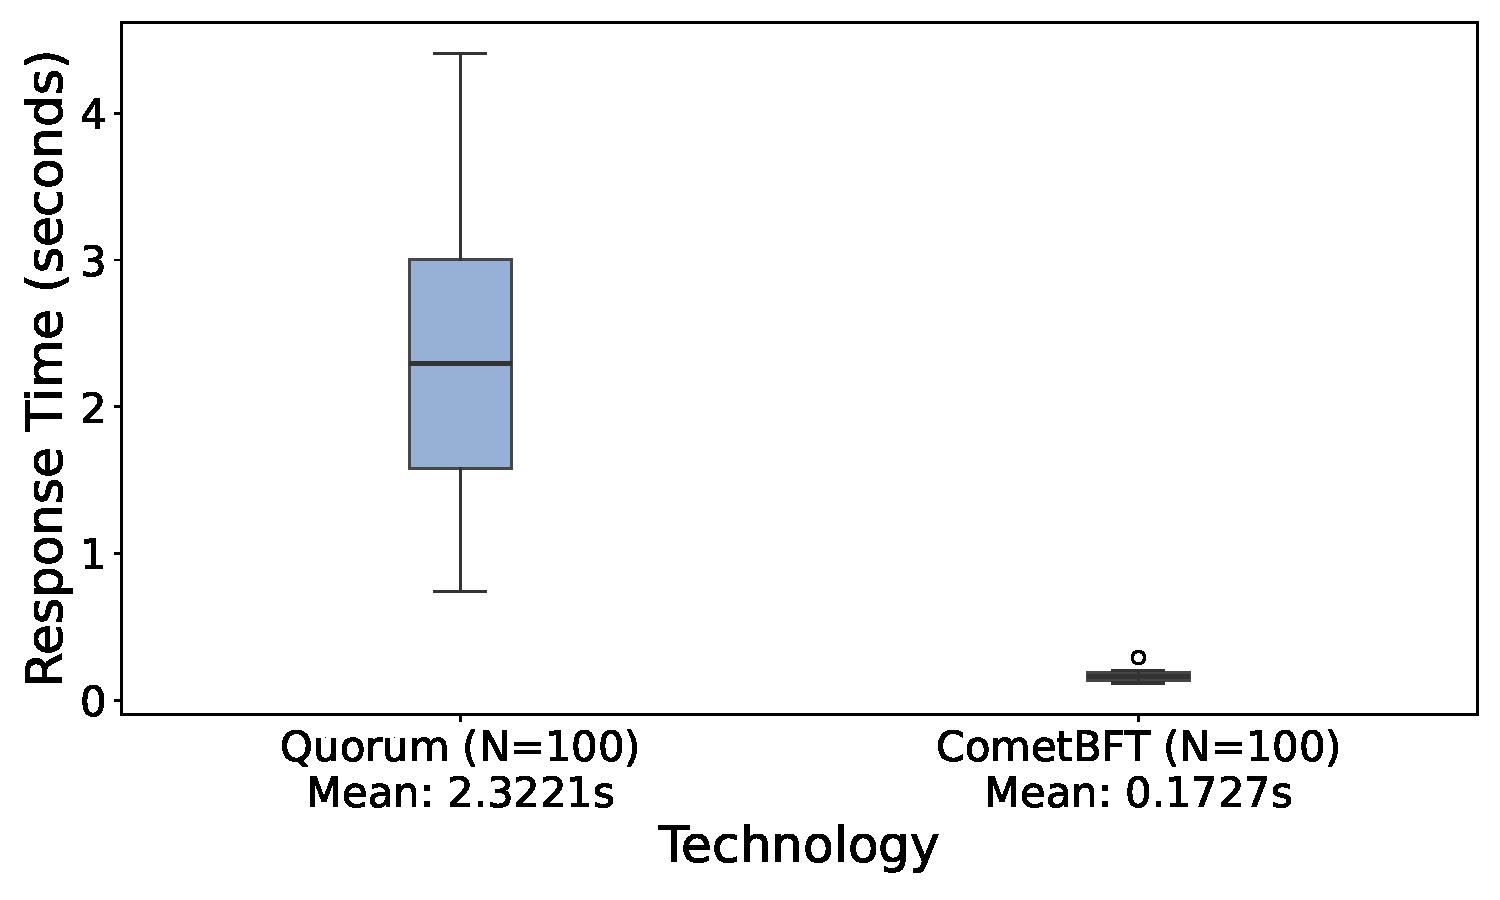
\includegraphics[width=0.72\textwidth]{Figures/Response_Time.pdf}
  \caption{Distribution of end-to-end response times in seconds under low traffic conditions for CometBFT and GoQuorum, over $100$ isolated-alert runs per backend. The mean response time is reported under each label.}
  \label{fig:resp_boxplot}
\end{figure}

Figure~\ref{fig:resp_boxplot} compares the distribution of end-to-end response times for the two configurations. The $x$-axis reports the evaluated technology together with its mean response time, while the $y$-axis reports the measured response time in seconds; for each configuration the box spans the interquartile range, the central line marks the median, and the whiskers represent the spread of the observations.

The results show a clear separation. CometBFT achieves a mean latency of $0.1727$\,s versus $2.3221$\,s for GoQuorum, an average response time roughly thirteen times lower. CometBFT also exhibits a markedly narrower interquartile range and a smaller overall spread, indicating more stable response times across runs, whereas GoQuorum shows both higher latency and greater variability. These results align with our prediction, GoQuorum's latency is bounded by all the tecnologic stack described in \chapter{requirement} such as the EVM and fixed minimum blocktime, CometBFT, by contrast, benefits from the on-demand block production, the first transaction is proposed immediately, the BFT round completes quickly on the validator set, and the state transition executes as a native Rust function call inside \texttt{DeliverTx} without bytecode interpretation or gas accounting.

From an SPS perspective this difference is both a performance and security relevant property. The liveness guarantee of Section~\ref{subsec:control_liveness} is bounded by the block production and execution latencies measured here, The experiment therefore empirically substantiates the qualitative claim that, under the sparse, event-driven alert traffic that characterizes a common SPS use case, CometBFT is lighter and more effective in supporting the requirements of the proposed architecture.


TODO DA QUI
% ==============================================================================
\section{Transaction Throughput under Increasing Load}
\label{sec:exp_throughput}
% ==============================================================================

% ------------------------------------------------------------------------------
\subsection{Motivation and Metric}
% ------------------------------------------------------------------------------

While Question~\ref{q:latency} characterizes the fixed cost per alert, Question~\ref{q:throughput} characterizes the variable cost under pressure. SPS workloads are not only sparse but also bursty: as noted in the burst-handling discussion of Chapter~\ref{chap:requirements} and in the deduplication rationale of Section~\ref{sec:impl_dedup}, a coordinated attack can trigger multiple IDS alerts within milliseconds, and a robust system must absorb these bursts without collapsing into unbounded latency or silently dropping alerts. The relevant metric is therefore the sustained transaction throughput of the ledger itself---the number of state transitions the consensus and execution layers can commit per unit of time---together with the latency required to drain a burst and the fraction of submitted transactions that are ultimately committed.

Throughput is a good metric for this comparison for two reasons. First, it stresses precisely the components that the requirement analysis flagged as divergent: the EVM execution and gas-metering loop that Quorum pays unconditionally, the fixed block period that bounds how quickly Quorum can drain its mempool, and, on the CometBFT side, the native ABCI execution path and the \texttt{CheckTx}-based mempool admission that allows the application to filter transactions before consensus (Section~\ref{subsec:impl_cometbft_app}). Second, it exposes the onset of performance degradation, which is where the architectural mismatch between a general-purpose platform and a narrow state machine becomes operationally visible: a backend that scales gracefully confirms that its overhead is intrinsic to the work being done, whereas a backend that collapses under load reveals overhead that is non-intrinsic and therefore, by the alignment lens of Section~\ref{sec:comparison}, a form of misfit.

\subsection{Experimental Design and Implementation}
\label{subsec:exp_throughput_design}

To evaluate the maximum throughput sustainable by the SPS, the harness progressively increases the input load by submitting transaction bursts ranging from $10^2$ to $10^5$ transactions, using up to $200$ parallel threads. For each burst size $N$ it measures (1) the number of transactions successfully committed to the blockchain, and (2) the elapsed time between the transmission of the first packet and the commitment of the last transaction. Throughput is then computed as the ratio between committed transactions and burst completion time, and the success rate as the ratio between committed and submitted transactions.

Two design choices are essential for fairness. First, the experiment injects transactions \emph{directly at the ledger's admission interface}, bypassing the IDS-to-member path, so that the measurement isolates raw ledger capacity rather than end-to-end attack handling; this is the regime in which the architectural difference between the two backends is cleanest. Second, the deduplication middleware of Section~\ref{sec:impl_dedup} is explicitly disabled on every node through the \texttt{POST /config/dedup} API for the duration of the benchmark, and the IDS alert path and the actuator feedback loop are muted. Disabling deduplication is necessary because its purpose is precisely to collapse redundant alerts into a single state transition; if it were active, the ledger would receive only a handful of transactions regardless of $N$, and the experiment would measure the middleware rather than the blockchain. Muting the IDS and the feedback loop prevents background traffic from contaminating the measurement. Both provisions are applied symmetrically and are reverted in a \texttt{finally} block at the end of the run, so that the lab is left in its default operating configuration.

The injection clients differ in transport but are matched in pressure. On CometBFT, a statically linked Rust binary (\texttt{sps-bench}) drives the validators through pipelined WebSocket \texttt{broadcast\_tx\_async} calls; on GoQuorum, a Node.js client (\texttt{quorum\_native\_bench.js}) drives the member nodes through concurrent \texttt{eth\_sendTransaction} calls with nonce resynchronization. Both use $200$ workers, a value well above each system's consensus throughput ceiling, so that the injection layer is never the bottleneck and the measured limit is genuinely the ledger's. After each burst the harness polls \texttt{/tx\_count} and the CometBFT \texttt{num\_unconfirmed\_txs} RPC until the chain reaches quiescence---a stable transaction count over several consecutive polls---before recording the final committed count and wall time; this ensures that transactions still in flight at the end of the burst are correctly accounted for rather than miscounted as lost.

\subsection{Results and Discussion}
\label{subsec:exp_throughput_results}

\begin{figure}[t!]
  \centering
  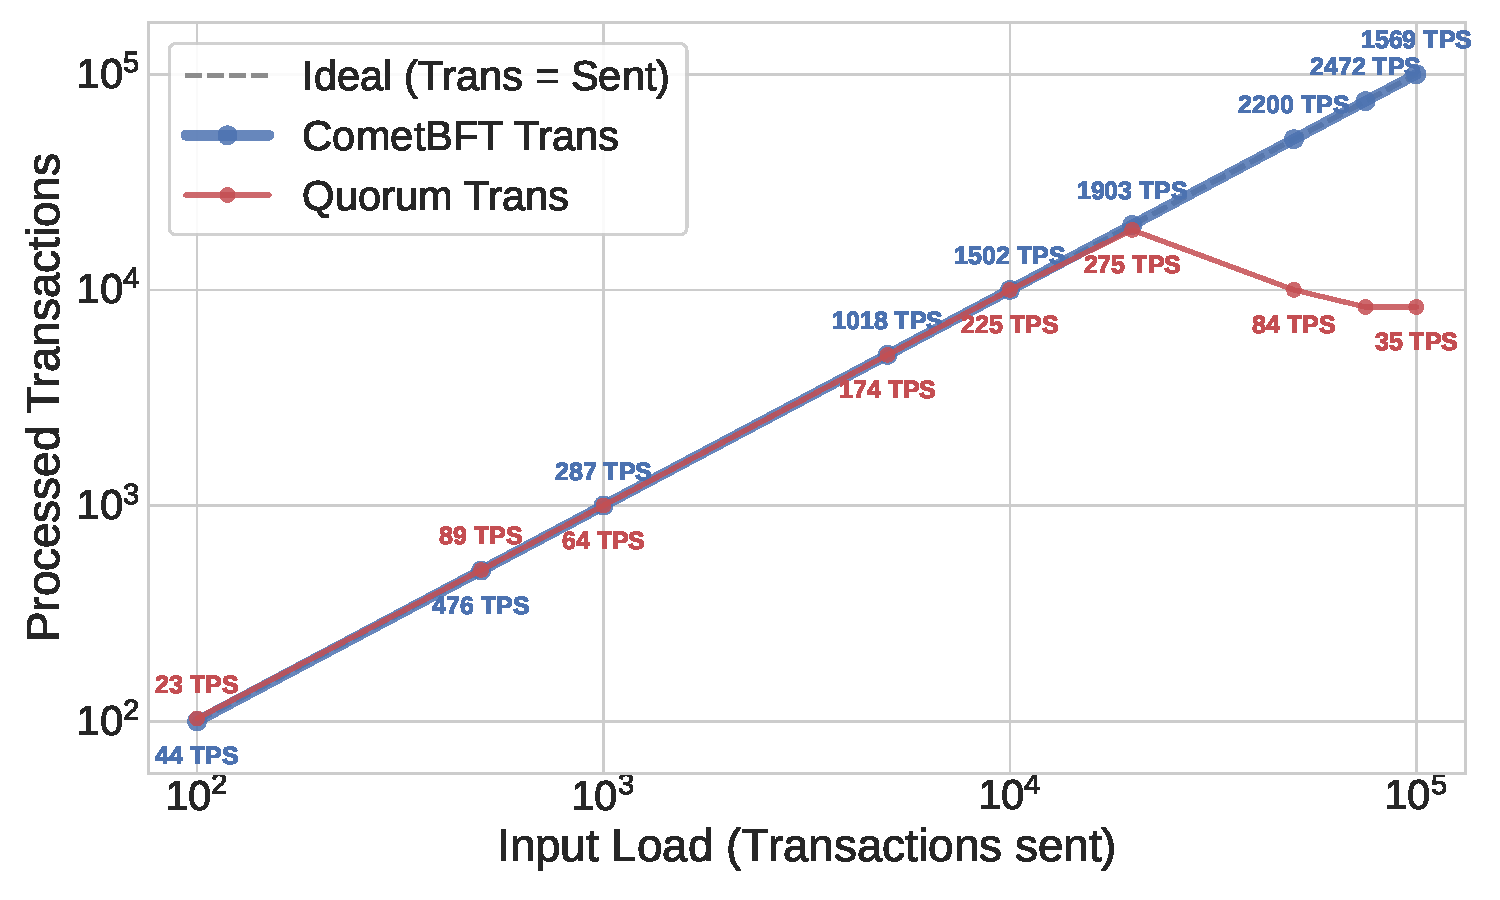
\includegraphics[width=0.78\textwidth]{Figures/comparison_transactions-1.pdf}
  \caption{Number of on-chain processed transactions as a function of the input load, on logarithmic axes, for the two blockchain configurations. The dashed diagonal is the ideal line (processed $=$ sent). Annotated values report the sustained throughput in transactions per second (TPS) at each load level.}
  \label{fig:throughput_trans}
\end{figure}

\begin{figure}[t!]
  \centering
  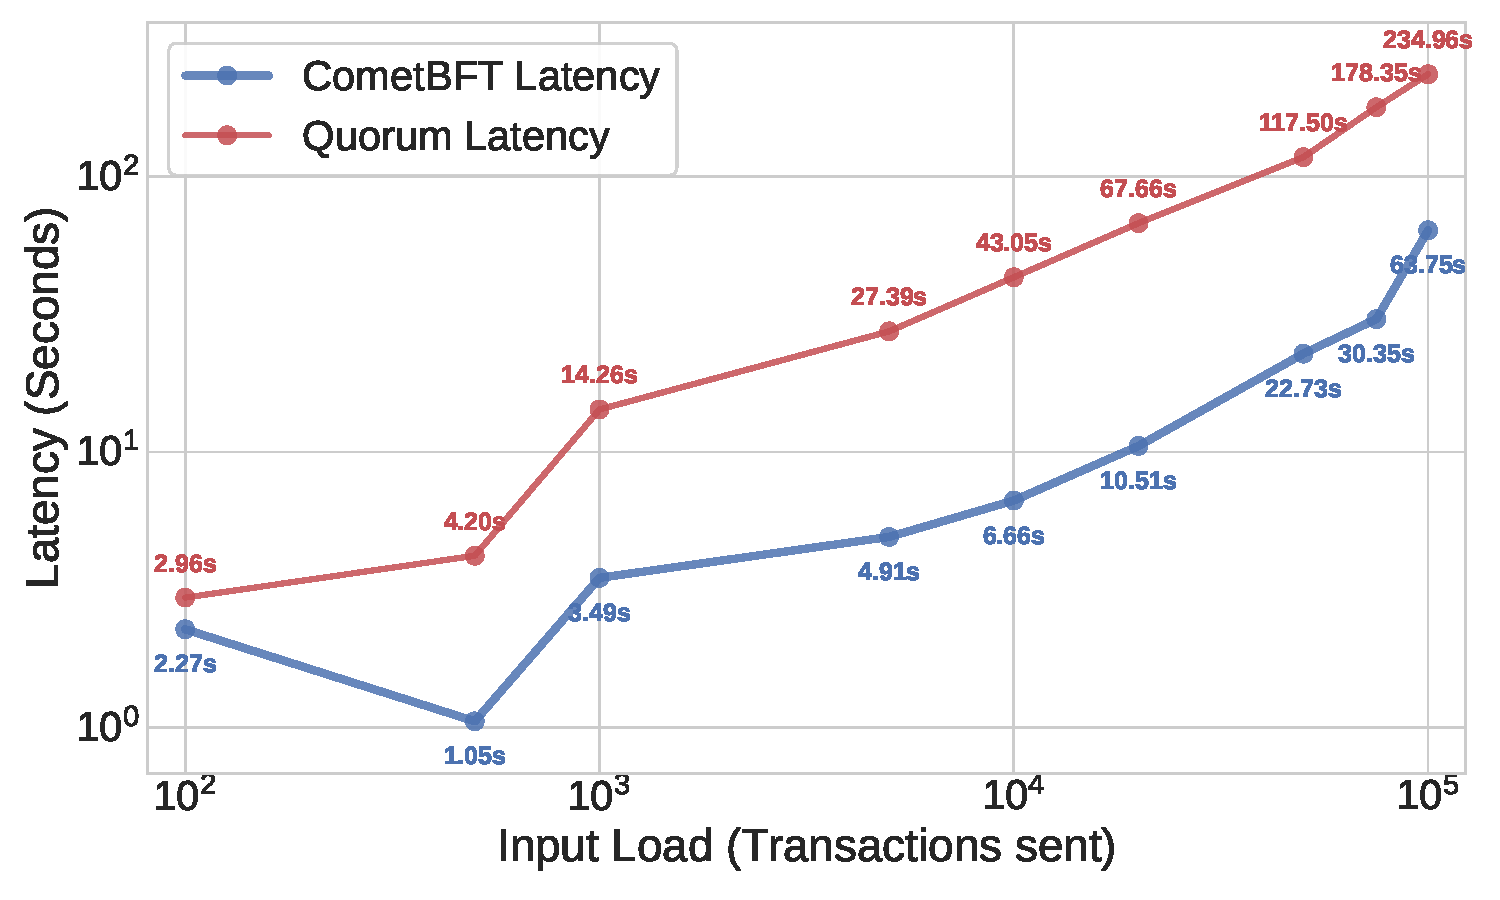
\includegraphics[width=0.78\textwidth]{Figures/comparison_latency.pdf}
  \caption{Burst completion latency as a function of the input load, on logarithmic axes, for the two blockchain configurations. Annotated values report the wall-clock time in seconds required to drain each burst.}
  \label{fig:throughput_lat}
\end{figure}

Figures~\ref{fig:throughput_trans} and~\ref{fig:throughput_lat} summarize the results from two complementary perspectives. Figure~\ref{fig:throughput_trans} reports, for each input burst, the number of transactions successfully committed on-chain against the ideal ``processed $=$ sent'' diagonal, annotating the sustained throughput in transactions per second (TPS); Figure~\ref{fig:throughput_lat} reports the wall-clock time required to complete each burst.

The results show a marked divergence. CometBFT scales effectively under increasing load: its committed-transaction curve tracks the ideal diagonal across the whole range, throughput rises from a few hundred TPS at low load to a peak of approximately $2.5$\,kTPS (the annotation reads $2472$~TPS) at the higher load levels, and no transaction loss is observed at any burst size. Latency grows accordingly from a few seconds to tens of seconds, reaching $63.75$\,s when submitting $100$\,K transactions, which is the expected price of draining a large burst through a fixed-size validator set with $O(n^2)$ voting communication (Section~\ref{subsec:validator_failure_quorum}). GoQuorum exhibits substantially weaker scalability. Throughput improves only under moderate load, peaking at approximately $275$~TPS for bursts of $20$\,K transactions, while latency increases sharply from seconds to several minutes, reaching $234.96$\,s at $100$\,K transactions---roughly $3.7\times$ the CometBFT figure for the same burst. At higher loads (above $10$\,K transactions) throughput collapses, with only about $10\%$ of submitted transactions successfully executed, and the committed-transaction curve detaches visibly from the ideal diagonal.

These outcomes map directly onto the requirement analysis. CometBFT's behaviour is consistent with the ``Execution model and deterministic state transitions'' discussion of Chapter~\ref{chap:requirements}: with the state machine implemented as a native Rust function inside \texttt{DeliverTx}, the per-transaction cost is proportional to the intrinsic logic of the transition rather than to virtual-machine scaffolding, and the \texttt{CheckTx} hook gives the application control over mempool admission. Combined with event-driven block production, this lets the ledger keep committing transactions as fast as the consensus round allows. GoQuorum's collapse is the empirical counterpart of the same analysis read in the opposite direction: every transaction pays RLP serialization, EVM bytecode interpretation, and instruction-granularity gas metering that execute unconditionally even though fees are zero; the fixed \texttt{blockperiodseconds=1} caps how quickly the mempool can drain; and once submissions outpace block production, the transaction pool fills and the success rate degrades. The higher CPU consumption observed on GoQuorum (Section~\ref{subsec:exp_resource}) is consistent with this interpretation: the extra cycles are consumed by the very machinery---gas accounting, EVM interpretation, on-chain governance---that the requirement table classifies as not needed.

From the SPS perspective, the decisive observation is not the raw peak throughput but the asymmetry in reliability under stress. CometBFT successfully executes \emph{all} submitted transactions across the entire range, whereas GoQuorum silently drops the majority of them once the load exceeds a few thousand transactions. In a self-protecting loop, a dropped alert is an unrecorded observation and, potentially, an unmitigated attack; a backend that sheds load by failing to commit transactions therefore undermines the liveness and auditability guarantees established in Sections~\ref{subsec:control_liveness}--\ref{subsec:act_safety}. The experiment thus corroborates, under sustained load, the same conclusion reached under low traffic: CometBFT better supports the SPS architecture, achieving higher throughput, lower delay, and---critically---no loss across all tested loads.

\subsection{Resource Consumption}
\label{subsec:exp_resource}

During the throughput benchmarks, user-process CPU utilization was monitored alongside the ledger metrics. On CometBFT, CPU utilization fluctuated between $9\%$ and $14\%$. GoQuorum exhibited slightly higher consumption, averaging $14\%$ and peaking at $17\%$. Although both figures remain modest in absolute terms---well below the $20\%$ ceiling observed throughout the campaign---the consistent gap is consistent with the architectural reading of Chapter~\ref{chap:requirements}: GoQuorum's higher resource usage is the runtime cost of the general-purpose virtual machine, gas accounting, and on-chain governance logic that the SPS does not need but cannot avoid, while CometBFT confines the trusted computing base to a small native state machine. This is the same mechanism that drives the latency and throughput gaps above, observed here in the dimension of energy and compute rather than time.

% ==============================================================================
\section{Effectiveness of the Deduplication Middleware}
\label{sec:exp_dedup}
% ==============================================================================

% ------------------------------------------------------------------------------
\subsection{Motivation and Metric}
% ------------------------------------------------------------------------------

The two previous experiments characterize the blockchain layer in isolation: Question~\ref{q:latency} at the single-alert extreme and Question~\ref{q:throughput} at the saturation extreme. The third experiment returns to the operating regime that the SPS actually faces in production---a regime in which a single sustained attack generates a large volume of redundant alerts that the system should not forward one-to-one to the ledger. As argued in Section~\ref{sec:impl_dedup}, a timed attack such as a sequence of SQL-injection attempts can produce hundreds of alerts per second, and three heterogeneous IDSs can each emit a matching alert within the same few milliseconds; since a BFT block commits on the order of seconds, the mempool would fill with thousands of redundant transactions describing the same state transition long before the first one commits, stalling consensus and inflating latency by orders of magnitude. The deduplication middleware was introduced precisely to prevent this, by dropping redundant alerts at the API level before they reach the mempool, since those redundant alerts would in any case be registered as a single response.

The metric of interest is therefore not throughput but \emph{compression}: how the number of transactions that actually reach the ledger scales with the volume of a specific attack, compared with the number of payloads sent, alerts detected, and alerts received at the blockchain-facing nodes. A good result is one in which the on-chain transaction count stays bounded---ideally constant---as the input load grows by orders of magnitude, while detection and ingress continue to scale. This directly tests the design goal stated in Section~\ref{sec:impl_dedup}: to keep the on-chain transaction load upper-bounded per block and per parameter, preventing mempool saturation while preserving the amount of information recorded. It also connects back to the broader architectural claim of Chapter~\ref{chap:requirements} that, in the SPS context, only state transitions matter and the relevant blockchain properties are minimality, determinism, and resilience rather than raw transaction capacity.

\subsection{Experimental Design and Implementation}
\label{subsec:exp_dedup_design}

Whereas Question~\ref{q:throughput} stresses the blockchain layer by disabling deduplication, this experiment enables it. The harness drives the attacker with \texttt{attacker\_burst.py} in \texttt{cycle} pattern, which sends the four canonical attack types (SQL injection, XSS, path traversal, command injection) in round-robin so that all four distinct state bits are exercised at every load level. The input load $N$ is progressively increased over four orders of magnitude. For each step the harness records four quantities:
\begin{itemize}
    \item \textbf{Sent}: the number of malicious payloads actually sent by the attacker;
    \item \textbf{Detected}: the number of alerts detected by the most virtuous IDS, taken as the maximum line count across the three IDS alert logs;
    \item \textbf{Ingress}: the sum of all alerts received at the blockchain-facing nodes, read from the \texttt{totalAlertsReceived} counter exposed by each node's \texttt{/stats} endpoint;
    \item \textbf{Transactions}: the number of transactions finally committed to the blockchain, read as the delta of \texttt{/tx\_count} between the beginning and the end of the run.
\end{itemize}

The experiment is run on the CometBFT configuration only. This is a deliberate, fairness-driven choice rather than an omission: with deduplication active, the number of transactions that reach consensus is so low that both backends behave equivalently, and a side-by-side comparison would measure experimental noise rather than an architectural difference. Focusing on a single backend keeps the figure legible while preserving the validity of the conclusion, which concerns the middleware rather than the consensus engine. Negative (recovery) alerts are suppressed for the duration of the run through a shared marker file consumed by \texttt{alert\_forwarder.py}, so that the deduplication cache is not reset between individual detections and the middleware can be observed over a sustained burst; between consecutive load steps, the harness sends a \texttt{SAFE\_ENVIRONMENT} reset to every light node, clearing both the ledger state vector and the per-node deduplication cache, so that each step starts from a clean baseline. Quiescence is enforced by polling \texttt{/stats} and \texttt{/tx\_count} until both stop growing before recording the final values.

\subsection{Results and Discussion}
\label{subsec:exp_dedup_results}

\begin{figure}[t!]
  \centering
  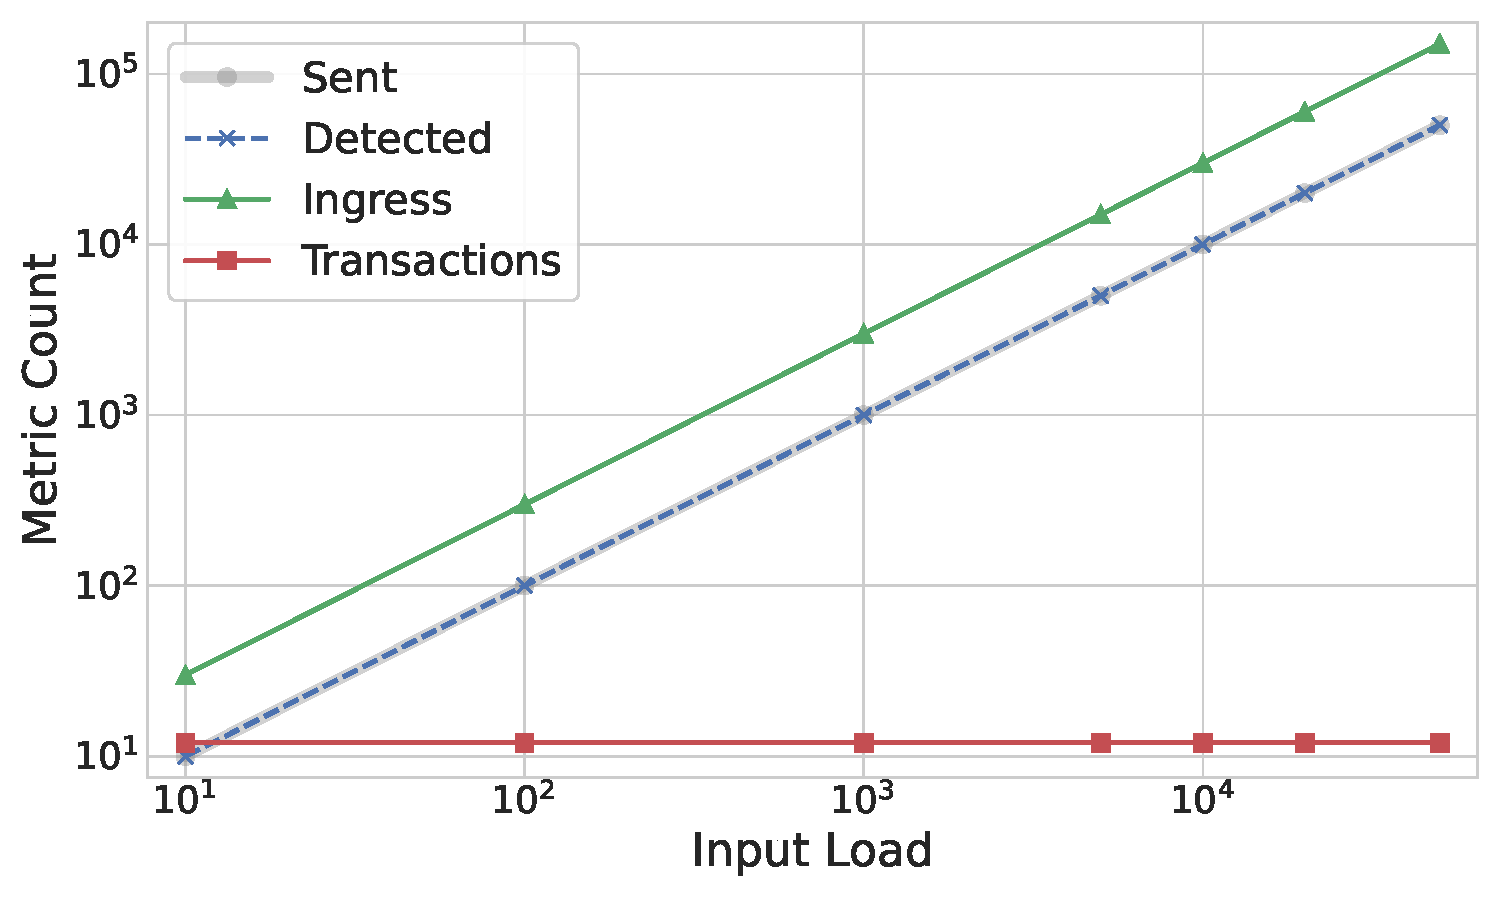
\includegraphics[width=0.75\textwidth]{Figures/SPS_comparison.pdf}
  \caption{Evolution of SPS processing metrics under increasing input load $N$, measured in attacks sent from the attacker machine: sent payloads, alerts detected by the most virtuous IDS, total ingress traffic received at the blockchain-facing nodes, and finalized blockchain transactions. Both axes are shown in logarithmic scale. Results are reported for the CometBFT configuration.}
  \label{fig:sps_dedup}
\end{figure}

Figure~\ref{fig:sps_dedup} is a multi-line plot showing how the four metrics evolve as the input load increases. The $x$-axis reports the input load $N$ and the $y$-axis the magnitude of each metric; both axes are logarithmic so that quantities differing by several orders of magnitude can be compared directly.

The results show that \textbf{Sent}, \textbf{Detected}, and \textbf{Ingress} all increase approximately proportionally with the input load, indicating that the attack-generation and detection stages scale consistently over the explored range and that the alert-forwarding path delivers the alerts to the blockchain-facing nodes without loss. In sharp contrast, \textbf{Transactions} remains essentially constant---flattening onto a single horizontal line on the logarithmic plot---even as the input load grows by four orders of magnitude. In the prototype this constant is bounded by the structural maximum $N_{\text{IDS}} \times N_{\text{types}} = 3 \times 4 = 12$ distinct state changes per step, which the middleware never exceeds regardless of how many redundant payloads the attacker produces.

This behaviour confirms the effectiveness of the deduplication middleware and closes the loop with several earlier claims. First, it validates the design rationale of Section~\ref{sec:impl_dedup}: because the consolidated state is a bit-vector and the response logic is a state--action map, any number of temporally adjacent alerts that request the same state change collapse into a single on-chain transition, so forwarding them individually would waste consensus cycles without altering the system's behaviour. By filtering redundant alerts at the API level before the mempool, the middleware keeps the on-chain load bounded per block and per parameter, which is exactly the property that prevents the mempool-saturation failure mode that Question~\ref{q:throughput} would otherwise expose. Second, it provides the operational complement to the requirement analysis of Chapter~\ref{chap:requirements}: the SPS does not need a high-throughput general-purpose ledger because the deduplication middleware, by exploiting the semantics of the state machine, ensures that the ledger is asked to commit only the transitions that actually matter. In this sense the experiment reframes the throughput result of Section~\ref{sec:exp_throughput}: CometBFT's multi-kTPS capacity is valuable not because the SPS routinely saturates it, but because it provides ample headroom above the bounded, deduplicated transaction rate that the system actually generates, so that even a misconfigured or partially defeated middleware is unlikely to stall consensus. Finally, the constant-transaction result confirms that the architecture preserves the full information content of the attack---which type occurred, confirmed by a quorum of heterogeneous IDSs---while shedding its redundant volume, which is the balance between auditability and efficiency that the ``configurable audit immutability'' discussion of Chapter~\ref{chap:requirements} anticipated.

Taken together with the latency and throughput results, the deduplication experiment completes the empirical picture. The SPS control loop reacts in fractions of a second on isolated alerts (Q1), sustains multi-kTPS bursts without loss when redundancy cannot be filtered upstream (Q2), and---in its intended operating regime---collapses four orders of magnitude of redundant attack traffic into a bounded, constant number of state transitions (Q3). Across all three regimes the CometBFT-based configuration exhibits the lower latency, higher throughput, and more predictable resource usage that the requirement-driven analysis of Chapter~\ref{chap:requirements} predicted, providing quantitative support for the thesis that an application-specific distributed state machine is a better fit for a cyber-resilient Self-Protecting System than a general-purpose smart-contract platform.
